\documentclass[a4paper, 11pt]{article}

\usepackage{natbib}
\bibliographystyle{agsm}
\setcitestyle{authoryear,open={(},close={)}}

\usepackage{fontspec}
\setmainfont[Ligatures=TeX]{Lato Light}

\usepackage{graphicx}
\usepackage{wrapfig}

\linespread{1.05}

\makeatletter
\renewcommand{\maketitle}{
\begin{flushright}
{\LARGE\@title}

\vspace{50pt}

{\large\@author}
\\\@date 
\vspace{40pt}
\end{flushright}
}
\renewcommand{\@seccntformat}[1]{}
\makeatother


\title{\textbf{The Impact of Digital Media on Urban Space and Media Facades}\\Piccadilly Circus}


\author{\textsc{Ans Vaessen}
\\13009722
\\{\textit{Digital Creativity and New Media Management}}}

\date{\today\\
word count: 3210}

%%%%%%%%%%%%%%%%% START %%%%%%%%%%%%%%%%%%

\begin{document}
\maketitle

\begin{abstract}
This essay examines the impact of digital media on the urban space by looking at the building facades and the use of new media. 
in particular 
and also 
change over the years from one way  communication to both ways....

\end{abstract}

\vspace{30pt} % Some vertical space between the abstract and first section

\section*{Introduction}



New media is everywhere, not only at home or on a smartphone it can be found in public places as well. There are many ways new media influence design. It can be in the way buildings or urban space are designed, developed, built and also literally on building facades, like the screens in Piccadilly circus.

This essay will give an overview of the literature on urban space, media facades and the interaction with the online world. Even if buildings are private-owned if they have a media facade they can still impact the public sphere.

One such building with a very famous facade is in Piccadilly Circus. Famous for being one of the first to have light advertisement. But also a good example of how facades change and influence the public space. With the development of new media the advertisement in Piccadilly circus changed as well and makes it a good case to look at the different theories relating to media facades, remediation and convergence to architecture.

Before looking at urban media, let's look at what makes urban media different from media in schools, offices or home. \cite{fritsch2008a} see different social and cultural practises when it comes to urban life compared to domestic life. \cite{Daalsgaard2010} see urban space as an arena for information systems.
That facades are changing is not a new phenomenon, architects always have been using new techniques, materials and ways to express themselves \citep{fritsch2008a}. Remediation of screens and facades in the urban area is a natural result of this urge to renew. 

\section{Growth urban facades} 
\cite{outdoor2009} state billboards are one of the oldest forms of advertisement and their numbers are still growing, outdoor advertisement is in China the fastest growing media form. In 2006 \$6.8 billion was spend on outdoor advertisement in the US and also in England expenses on outdoor commercials grew with more than \pounds 250 million between 2001 and 2006 \citep{outdoor2009}. \cite{outdoor2009} continue to explain outdoor advertising is growing, because it is harder to reach an audience through the traditional media like television, radio and print. Using outdoor advertisements can help to catch the 'consumers on the go' the passer-by can not block it or skip the commercials \citep{outdoor2009}. Furthermore the quality of screens has been improving from illuminated advertising signs to led display so more is possible \citep{outdoor2009}.

\cite{outdoor2009} Predicts outdoor advertisement will continue to grow and diversify as it is one of the best ways to reach the desired audience and integrate market communication, this despite the anti-billboard sentiments.

\section{remediation in urban places}



\subsection{Urban screens and convergence to architecture}


Architecture and media technology are melting in each other claims \cite{Slaatta2006}, a convergence of buildings and new media is taking place. As mentioned earlier architecture is always renwing itself and changing the landscape.\cite{Slaatta2006} describes how the urban landscape changed and with the new screen technology becomes the new landscape, and furthermore how it diffuses the border between natural and electronic landscape. “The intentional use of digital screen technology in transparent or fluorescent building materials for projection of digital images on building facades is changing the meaning of both media and architecture” \citep[P.1]{Slaatta2006}.

An other phenomenon is the way the meaning of cultural work itself is changing media. Traditionally the national broadcaster was responsible for the content on television and one would watch television at home. 

Today we watch everywhere and content is coming from different sources as well.\cite{shirky2010} points our, watching television is no longer one way, everybody is participating and even uploading material mainly on social media and websites like Youtube.
To explain this better \cite{Slaatta2006} makes a comparison with Charlie and the Chocolate Factory. ..."The imagined situation is parallel to the technological vision in the film version of Roald Dahls famous novel Charlie and the Chocolate Factory, where both objects and persons are made able to move between the physical world and the television screen world. Not only does a chocolate bar suddenly appear in Stanley Kubricks 2001: A Space Odyssey. But also Mike Teavee, the incarnated adolescent television consumer, is inserted in a news program. Although there is some slight physical distortion, the technological experiment shows that "it works"... \citep[P.1]{Slaatta2006}.

\cite{Slaatta2006} observes that these new strategies of amusement and amazement draw people to non-existence place on the screen, the traditional way of live broadcasting disappears and you are participant, producer and viewing yourself at the same time. Furthermore \cite{Slaatta2006} argues that the architecture and audiovisual convergence also questions the border between urban and suburban.

The screen itself becomes the landscape, it can even use reflection or camouflage and it integrates with its environment \cite{Slaatta2006}. When the screen is invisible it can imitate a surface or reflect its surroundings like skyscrapers, with glass windows, mirroring the nearby buildings floors, windows and decorative elements \citep{Slaatta2006}. Standing out according to \cite{Slaatta2006} there are active visual borders, displaying advertisement or showing SMS texts.

\subsection{New media and cyberspace in the urban space}

Lastly it is interesting to look at \cite{Graham} comments on new media and the information society, the common believe that new media would undermine geographical concentrations in cities has turned out to be not true.

( He is of the opinion the new media and urban environment support each other and found a place in the urban studies as a sort of subdiscipline \cite{Graham} coins as ‘urban new media studies’.)

Furthermore he explains that remediation of everyday urban life is not replacing old media but using it in different ways, remediate traditional media like TV, newspapers, books, art and so on. In his paper 'beyond the dazzling light' he makes a couple of points to analyse the remediation of urban life \citep{Graham}. In this essay a couple of these points will be further examined and used to analyse the example of Piccadilly Circus.

Firstly the relationship between the new media and the old media, infrastructure, technologies and space is still strong, there is no radical break with the past \cite{Graham}. He goes on to note, the online world or cyberspace is a also a remediation of the real world \cite{Graham}.

An other notable observation is banalization, when the novelty wears off, new media is no longer new and become less visible. This already happening with the way it is embedded in everyday life and less and less visible, \cite{Graham} gives the example of electricity or water, no-one gives it much thought. This also touches on what \cite{bolter2003} describe as the myth of transparency to get the user as close as possible to the real thing. Not banalization but so real it is overlooked or transparent like a window and not noticed, \cite{bolter2003} remark that interaction with the media can be described as a mirror.

A last point made by \cite{Graham} is the growing invisibility of sociotechnical power, he gives a basic example about call liner identifcation, phone systems that judge if the caller is a 'good' or 'bad' customer and based on that needs to wait in the short or long queue. Today the hazard with data and sociotechnical power are even bigger and better hidden. 


The theories above are used to analyse the case of Piccadilly circus. 


\section{Piccadilly Circus}


One of London's busiest public urban places is Piccadilly Circus, with around 100 million people passing through it each year, this is a prime spot for brands to advertise \citep{Dezeen}.

The advertisement on Piccadilly is more than 100 years old. An overview in the \cite{telegraph2011} shows the first illuminated advertisements dates back to 1908. Later \cite{nelson1998} writes at the end of the millenium how the lights are moving with time and switching to digital billboards. Managing Director of the design house Sedley Place Mick Nash is cited in the article saying: "It blends art, science and commerce. We have called it Street Vision because it is a whole new way of talking to the public. It is not TV and not a poster, but a new type of media which cuts across those two"\cite{nelson1998}.

After more than 100 years the place 'Piccadilly Circus' becomes synonymy with the screens on the surrounding buildings, it is part of the landscape. As \cite{Slaatta2006} argued earlier the border between urban and suburban is disappearing. The points made by \cite{Graham} can be applied to the media facade in Piccadilly Circus. The new media on the screens doesn't break with the old, it is still outdoor advertisement but displayed differently. Furthermore the screens on Piccadilly Circus risk to become banal for two reasons, screens are not novel any more and neither is advertisement. Since we see so much of it nowadays it almost turns into a window, people don't notice it any more.

This of course is a problem for the companies advertising, The screens are there to capture the audience. As touched upon earlier outdoor advertisement is still growing, probably as we will see because it is also changing and remediating as we will see. 

Three examples used on the screens on Piccadilly circus in the past will illustrated how new media changed the billboards designs.

\subsection {Interacting with the billboard}

The first example dates from 2009 and is a McDonald's interactive LED billboard, created by Leo Burnett, still and moving, iconic images are displayed for 40 seconds, to allow people to take pictures interacting with the images, like holding flower as shown on picture \ref{fig:graph1} \citep{campaign2009}. 

\begin{figure}[h!]
    \centering
    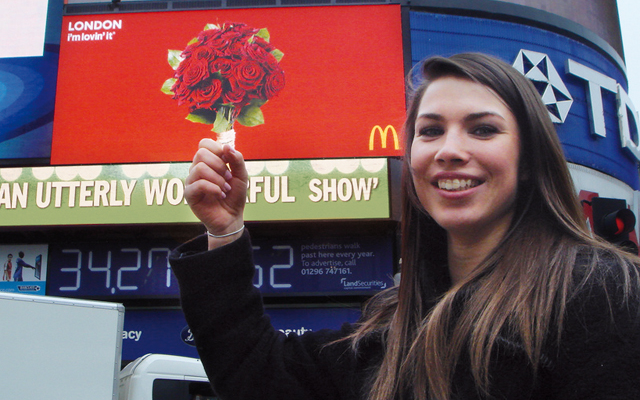
\includegraphics[width=0.9\textwidth]{weights.png}
    \caption{Interacting with the billboard \citep{campaign2009}}
    \label{fig:graph1}
\end{figure}

Mc Donalds encourage people to interact with the billboard, take poses with a bowler hat or umbrella, or say hi to you mum on Mother's Day, to spread the message you can post you pricture or video on social media like Facebook, Flicker or You Tube, spreading the McDonalds Logo over the web (see youtube video \citep{youtube2009}).  

This example is remediation of the billboard, not static advertisment, instead the pictures are changing and challenging the visitors of Piccaidlly circus to interact with it. The screen is not part of the landscape it is 'standing out', as \cite{Slaatta2006} describes it, by enganging people. Besides that the advertisement is send into the cyberspace, but the content is rooted partly in a real place -picadilly circus- and partly on a screen anywhere, as long as one has access to social media the picture can be seen.  

An other observation is that the spectator is no longer looking at a screen as looking through it as a window, because you need to interact with, strike a pose, it reflects as a mirror, because the pictures depict both you and the billboard.


\subsection {Being part of the billboard}
Moving forward to 2014 the technique improved and McDonald's launched a new campaign to put people on the screens and become part of the screen see \ref{fig:graph2}. This fictional world was called 'little Piccadilly', people passing the screen were invited to create there own avatar on LittlePicca.com and send it to the screen through their smartphone, with 300 million different combinations and real-time weather reflecting the actual weather, you will never see the same thing twice \citep{youtube2015}. 

\begin{figure}[h!]
    \centering
    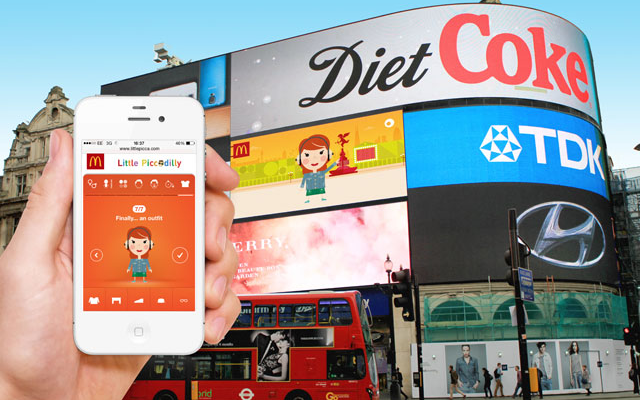
\includegraphics[width=0.9\textwidth]{avatar.png}
    \caption{Being part of the billboard \citep{campaign2014}}
    \label{fig:graph2}
\end{figure}

Nathalie Pomroy, the director of marketing at McDonald’s, said: "We have embraced recent innovations in the digital media field, and as new trends develop and as the interactive media industry reaches maturity, we will continue to look for innovative ways to communicate with our customers" \citep{campaign2014}.

Again a good example of remediation and how new media influenced the design and tries to stand out. Once more there is a parallel with the windows and mirror metaphor \cite{bolter2003} use. Using an avatar people are waving back at themselves from the big screen in Piccadilly Circus. With an avatar you yourself become part of the landscape and we almost like Mike Teavee as we saw earlier \ref{Urban screens and convergence to architecture}. With this new way of engaging people McDonald's brought a new novelty to outdoor advertisement and prevented banality and becoming invisible. 

\subsection {The billboard is looking at you}


New digital billboards installed in 2017 use recognition technology, so the screens display targeted commercials based on the people visiting Piccadilly Circus \citep{Dezeen}. \cite{Dezeen} notes that brands can send specific advertisement to the passer-by, using make, model and colour of the cars or age and gender of the pedestrians. The camera combined with algorithm data can make assumptions on visual cues such as hair length and hight to guess the demographics of the area and for instance, display promotions for womenswear if there are more women in the area \citep{Dezeen}. The adverts can be further specified depending on weather, news, sports and social media updates \citep{Dezeen}. However Landtec the owner of the screen is quick to point out "Although the Piccadilly Lights screen will be able to display advertising content that responds to real-time factors – such as the weather or the colour of cars – the technology is not able to recognise individual people or display individually targeted content."

An other change was a new screen that replaced the old screens, these were divided in six panels, the screen is wrapped around the building and can show one advertisement as shown on \ref{fig:graph3} but can still display different advertisements at the same time, this is something they weren't able to do before, because the six screens were made by different manufactures \citep{wired}.

\begin{figure}[h!]
    \centering
    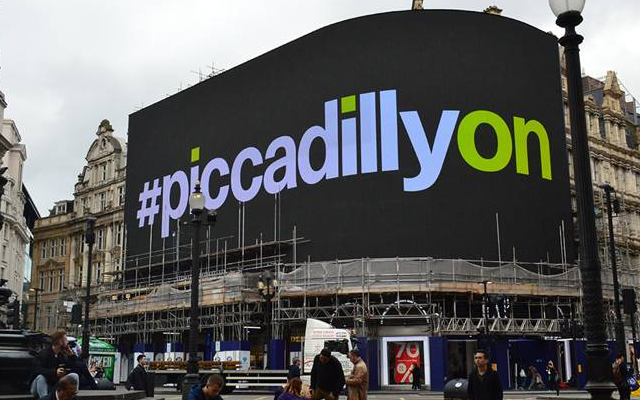
\includegraphics[width=0.9\textwidth]{on.png}
    \caption{One big screen \citep{wired}}
    \label{fig:graph3}
\end{figure}

This example refers to on an other point made by \cite{Graham} about the sociotechnical power that is often hidden. The fact that we are guided in what advertisements we get to see, not the same for everybody. This raises the question were this will lead.



\subsection{Critical reflection}

First of all the notion that new media can become part of the urban landscape seems true for Piccadilly Circus. Like Slaatta said: "The screen technology itself is becoming a landscape" \citep{Slaatta2006}. In this case one might even argue the screen is shaping the landscape, the billboard on Piccadilly Circus is not only part of the landscape it is one of the landmarks and tourist attractions in London. People go to this place to look at the famous billboard. 

Looking at the new media in the urban environment the screens in Piccadilly Circus is a good example, since they have been there for more than 100 years it is possible to look at the changes over the years. Which is the first point made by \cite{Graham}, that new media is not so different from old media, but merely remediating the old. In other words giving the old billboard a face-lift. 

It turns out that this face-lift is a necessity, the main goal for the billboards on Piccadilly Circus is not to be a tourist attraction but to find an audience, to be noticed. As \cite{Graham} puts it, new media is prone to become ordinary, invisible maybe. Advertising agencies like Leo Burnett have to come up with new ways to engage people with the brand. The display itself changes as well, the quality is improving from illuminated billboards to one big screens that can be split in small ones.

The interaction with the billboards and the use of new media like smartphones is more remediation and shifting between cyberspace and real places. \cite{Graham} points out most traffic of digital information takes place in urban areas and also the communication often is limited to those in your own area. In this case showing a photo of you on Piccadilly Circus to your friends back home. Even better making an avatar at home and sending it to the screen in Piccadilly Circus via LittlePica.com. 

It is not invisible it stands out, the metaphor \cite{bolter2003} use is already mentioned. But at the same time for a lot of Londers who travel through Piccadilly Circus every day, more is needed to turn their gaze up and change the window into a mirror. One that got heads turned was the display for Armistice centenary, an experience with light and sound and video on the new big screen, to commemorate the soldiers who fought and died in the Great War \cite{drum}. But it is hard to find other cases that had the same effect in recent years.

Lastly with the recent development of a screen that is watch the audience we enter yet another era and \cite{Graham} points out the sociotechnical power is growing invisible. And even after reading Landtec's statement that it is facial dedectation and not facial recognition \citep{landtec}. It still makes one wonder how much they see if they can even see the mood (based on whether think you are frowning or laughing) and they claim not to save any of the images but what if someone else gets in \cite{landtec}. From the comments on the articles \citep{Dezeen} it becomes clear people are not happy with this intrustion in their privacy.



\section{Conclusion}

Looking back at the stages Piccadilly Circus billboard gone through from light up displays to moving pictures and interacting with the public \citep{outdoor2009} was right with his predictions, that the outdoor advertisement would keep on growing. It is probably still one of the best ways to get an audience attention. It also shows how new media had an impact on designing facades and what the influence is on the urban space and cyber space. New media is remediated and connected to other media like smartphones and social media.

The billboards on Piccadilly circus are part of the landscape and for some are almost invisible because they are always there, for others it stands out it is a tourist attraction and invites them to interact. So depending on the audience a window or a mirror.

However with the hidden camera's behind the display the audience is targeted with specific advertisements and it is clear not everybody is happy with this development and it is important to be aware about this even when one can not see it. 






%% disable some things
\renewcommand{\textbf}{}
\renewcommand{\bf}{}
\bibliography{biblio}{}
\end{document}
